% title: Pushforward adds input and output changes
% description: The original IR maps inputs to an output. Pushforward adds an input-change channel and an output-change channel. Both channels run forward.
% width: 32rem
\documentclass[tikz,border=5pt]{standalone}
\usetikzlibrary{arrows.meta}
\begin{document}
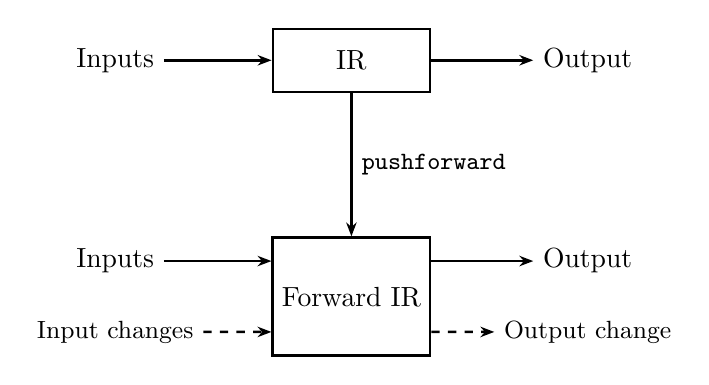
\begin{tikzpicture}[
    box/.style={draw, line width=0.8pt, minimum height=0.8cm,
                minimum width=2cm, align=center},
    flow/.style={-{Stealth[length=5pt]}, line width=0.9pt},
    note/.style={font=\small, align=center},
]

    \node[box] (original) at (3, 0) {IR};
    \node (inputs) at (0, 0) {Inputs};
    \node (output) at (6, 0) {Output};
    \draw[flow] (inputs) -- (original);
    \draw[flow] (original) -- (output);
    \node[box, minimum height=1.5cm] (new) at (3, -3) {Forward IR};
    \draw[flow] (original.south) -- node[right, note] {\texttt{pushforward}} (new.north);
    \node (newin) at (0, -2.55) {Inputs};
    \node[note] (changein) at (0, -3.45) {Input changes};
    \node (newout) at (6, -2.55) {Output};
    \node[note] (changeout) at (6, -3.45) {Output change};
    \draw[flow] (newin.east) -- ([yshift=0.45cm]new.west);
    \draw[flow] ([yshift=0.45cm]new.east) -- (newout.west);
    \draw[flow, dashed] (changein.east) -- ([yshift=-0.45cm]new.west);
    \draw[flow, dashed] ([yshift=-0.45cm]new.east) -- (changeout.west);
\end{tikzpicture}
\end{document}
